\chapter{Datensatz}
\label{chap:Datensatz}
In dem Praxisprojekt, auf das diese Bachelorarbeit aufbaut, wurden Bewertungen von Anwendungsregeln aus vorherigen Projekten der Siemens Mobility GmbH gesammelt und in eine CSV-Datei geschrieben.
Wie im Kapitel \ref{chap:Keras} beschrieben, ist der erste Schritt beim Erstellen eines \ac{DL}-Modells als \ac{NN} das Definieren des Datensatzes sowie die Aufteilung
dessen in Eingabe- und Ausgabewerte. Dieses Kapitel wird sich mit diesem Schritt beschäftigen und den Datensatz so aufbereiten, dass er für das Anlernen des \ac{KI}-Modells genutzt werden
kann. Zudem werden in diesem Kapitel wichtige Eigenschaften des Datensatzes visualisiert.

\section{Datensatz aus dem Praxisprojekt}
\label{chap:DataPraxisprojekt}
Das Ergebnis aus dem Praxisprojekt war ein Datensatz mit 195.518 Bewertungen zu Anwendungsregeln. Beim Erstellen des Datensatzes wurde jedoch ein entscheidender Fehler begangen.
Als die Daten aus den Projekten gesammelt wurden, wurde dabei auch jede Baseline eines Moduls berücksichtigt ohne zu überprüfen, ob sich an der Anwendungsregeln und ihrer Bewertung
etwas geändert hat. Die Folge dessen war, dass der Datensatz eine Vielzahl von Duplikaten enthalten hat, was dazu geführt hätte, dass Projekte mit mehreren Baselines 
stärker ins Gewicht gefallen wären, obwohl die Anzahl an Baselines nichts über die Signifikanz der Bewertung aussagt. Deshalb mussten die erstellten Module mit den bewerteten Anwendungsregeln
in \ac{DOORS} überarbeitet werden. 

Dafür wurde ein Skript in \ac{DXL} geschrieben, was in den Modulen nach Duplikaten sucht und diese löscht. Die äußere Schleife durchläuft dazu alle 
Elemente in dem Ordner, in welchem sich die Module mit den bewerteten Anwendungsregeln befinden. Wenn ein Element ein Formal Module ist, 
dann wird dieses Modul geöffnet und in einer inneren Schleife werden alle Objekte des Moduls durchlaufen. Für jedes Objekt wird eine 
Zeichenfolge erstellt, die aus den Attributen ObjectText, Status und Statement besteht. Anschließend wird überprüft, ob diese Zeichenfolge
in einer Skiplist bereits vorhanden ist. Wenn dies der Fall ist, dann wird das Objekt als Duplikat erkannt und mittels der softDelete()-Funktion
als gelöscht gekennzeichnet. Wenn diese Zeichenfolge noch nicht in der Skiplist vorhanden ist, dann ist dieses Objekt noch einzigartig und wird der Skiplist
hinzugefügt, um sicherzustellen, dass zukünftige Duplikate erkannt werden. Anschließend wird die Zeichenfolge geleert. Nachdem die innere Schleife durchlaufen wurde,
werden alle Objekte, welche als gelöscht gekennzeichnet wurden, endgültig aus dem Modul entfernt. Zudem wird der Inhalt der Skiplist entfernt, bevor das nächste Modul durchlaufen wird, um 
zu gewährleisten, dass diese bei der nächsten Verwendung keine Elemente aus vorherigen Modulen mehr enthält.

\begin{lstlisting}[language = C++, caption={Duplikate in Modulen löschen},captionpos=b, label = lst:deleteDuplicates, float, floatplacement=H]
    // ...
    for it in f do{
        if (type(it) == "Formal"){
            m = edit(fullName(it), false)
            for o in entire m do{
                szData = o."ObjectText""" o."Status""" o."Statement""";
                if(find(slUnique, szData)){
                    softDelete(o);
                }else{
                    put(slUnique, szData, szData)
                }
                szData = "" 
            }
            purgeObjects_(m)
            delete(slUnique)
        // ...
\end{lstlisting}

Das Entfernen der Duplikate hatte zur Folge, dass der im Praxisprojekt gesammelte Datensatz von ursprünglich 195.518 auf 14.572 bewertete Anwendungsregeln reduziert wurde.
Der Grund, weshalb der Datensatz auf rund 7,5 \% seiner eigentlichen Größe geschrumpft ist, liegt darin, dass einige Projekte bis zu 40 Baselines hatten, 
wo sich aber die meisten Anwendungsregeln nicht verändert hatten. Dieser Schritt war wichtig, um dafür zu sorgen, dass bestimmte Bewertungen nicht stärker gewichtet werden,
als andere. \\

Nun besteht der Datensatz aus 14.572 Einträgen, die jeweils aus drei Attributen, nämlich dem eigentlichen Text der Anwendungsregel sowie dem Status und dem Statement bestehen.
Wie in der Abbildung \ref{fig:Programmierparadigma} dargestellt, benötigt ein Modell Eingabedaten und die dazugehörigen Antworten. Die Eingabedaten stellen in diesem Fall
die Texte dar, während die Antworten hier in Form des Status und des Statements dargestellt werden. Angenommen der Status einer Anwendungsregel X wird 15-mal mit closed
und zehnmal mit open bewertet und ein Modell wird mit diesen Daten angelernt. Würde ein neues Projekt nun diese Anwendungsregel X importieren und einen Vorschlag vom Modell
generieren lassen, dann würde das Modell eine Mehrheitsentscheidung durchführen und prüfen, wie oft die Anwendungsregel in der Vergangenheit mit welchem Status bewertet wurde.
Das Modell würde aufgrund der Mehrheitsentscheidung diese Anwendungsregeln immer mit closed bewerten. Das wäre ein legitimer Ansatz um Vorschläge zu generieren. 
Dahinter steckt jedoch lediglich keine Struktur, die das Modell erkennen könnte, und somit auch keine Intelligenz. Dieses Problem könnte auch mit einer einfachen Tabelle 
gelöst werden, das Nutzen eines \ac{NN} wäre hier unnötig. Daher benötigt der Datensatz noch weitere Attribute, da die Bewertung von Anwendungsregeln nicht alleine durch die 
reine Anzahl an Bewertungen in der Vergangenheit prognostiziert werden kann. Beispielsweise spielen regionale Gegebenheiten eine große Rolle, 
da wenn Projekte im selben Land durchgeführt werden, es wahrscheinlicher ist, dass sie Anwendungsregeln ähnlich bewerten. 

Um an mehr Daten über die vorherigen Projekte zu gelangen, muss das Skript aus dem Praxisprojekt erweitert werden. Neben dem Text der Anwendungsregel, dem Status und dem Statement
muss auch das Produkt und die Version der Komponente berücksichtigt werden, von der die Anwendungsregel stammt. Ebenso spielt der Name des Projekts eine Rolle,
da durch ihn in Kapitel \ref*{chap:DatenSammeln} in einer Access-Datenbank nach Informationen zu dem Projekt gesucht werden kann. 
Das Produkt und die Version der Komponente lässt sich durch den Link bestimmen, den jedes Objekt auf das zentrale Projekt hat, in der die Anwendungsregeln gespeichert werden.
Dieses Projekt heißt RA Application Conditions und ist dabei wie folgt aufgebaut:

\begin{quotation}
    $\textbackslash$RA Application Conditions$\textbackslash$XX\_PG$\textbackslash$Kategorie$\textbackslash$Produkt\dots
\end{quotation}

Aus dem Zielobjekt des Links lässt sich das Modul bestimmen, in dem die jeweilige Anwendungsregel gespeichert ist. Das Modul trägt dabei als Namen die Versionsbezeichnung eines Produkts.
Über den Speicherpfad lässt sich außerdem das Produkt, als das dritte Element des Pfades, bestimmen. Im \ac{DXL}-Skript muss also eine weitere Schleife hinzugefügt werden.
Diese Schleife soll alle ausgehenden Links eines Objekts durchlaufen, bis ein Link gefunden wurde, dessen Zielobjekt sich im Projekt RA Application Conditions befindet.
Wenn so ein Link gefunden wurde, dann wird der vollständige Pfad an eine selbstgeschriebene Funktion übergeben, die als Rückgabewert den Namen des Produkts hat.
Außerdem wird die Versionsbezeichnung ebenfalls dem Link entnommen und in einer Variable gespeichert. Dabei ist zu beachten, dass die Funktion target(Link) überladen ist.
Im ersten Fall wird eine Referenz auf das Modul zurückgegeben, auf das der Link zeigt. Diese Referenz beinhaltet den kompletten Pfad. Im zweiten Fall wird lediglich der Name des Zielmoduls 
zurückgegeben \cite[vgl. S.391]{DXL}. Da der Name des Moduls bereits die Produktbezeichnung beinhaltet, ist hier der volle Pfad nicht relevant.

\begin{lstlisting}[language = C++, caption={Produkt- und Versionsbezeichnung bestimmen},captionpos=b, label = lst:getProductVersion, float, floatplacement=H]
    // ...
    for l in all o -> "*" do{
        mnTarget = target(l)
        if(fullName (getParentProject(mnTarget)) == fullName (project("RA Application Conditions"))){
            szProduct = getProduct(target(l)) 
            szVersion = target(l)
            break;
        } 
    }
    // ...
\end{lstlisting}

Während des Praxisprojekts wurden alle bewerteten Anwendungsregeln nach Projekt und Komponente gruppiert. Dabei liegen alle bewerteten Anwendungsregeln eines Projekts jeweils in einem Ordner.
Der Name dieses Ordners trägt den Namen des Projekts. Um nun an den Namen eines Projekts zu kommen, muss lediglich der Name des Ordners geprüft werden, in dem sich das aktuelle Modul befindet.
Dies wird ermöglicht durch die getParentFolder()-Funktion, wie dem Quellcode \ref*{lst:getPath} entnommen werden kann. In der Access-Datenbank steht vor dem Namen des Projekts noch ein 
Slash, weshalb dieser noch vor den Namen gesetzt werden muss.

\begin{lstlisting}[language = C++, caption={Projektnamen bestimmen},captionpos=b, label = lst:getPath, float, floatplacement=H]
    // ...
    for it in f do{
        if (type(it) == "Formal"){
            m = edit(fullName(it), false)
            Folder fParent = getParentFolder(it)
            String szPath = "/" name fParent
            // ...
\end{lstlisting}

Das Ergebnis dieser beiden Schritte ist eine CSV-Datei mit 14.572 Einträgen, die jeweils 6 Attribute (Text der Anwendungsregel, Produkt, Version, Pfad, Status, Statement) besitzen.
Diese Datei kann nun mittels der Pandas-Bibliothek in ein Python-Skript importiert werden.

\section{Importieren des Datensatzes}
Um die Pandas-Bibliothek zu nutzen, muss diese zunächst importiert werden. Beim Importieren einer Bibliothek besteht die Möglichkeit dieser Bibliothek einen Alias zuzuweisen,
wie in Zeile 1 des Quellcodes \ref*{lst:importData} zu erkennen ist. Für die Pandas-Bibliothek ist dabei pd als Alias gebräuchlich.

\begin{lstlisting}[language = python, caption={Pandas und den Datensatz importieren},captionpos=b, label = lst:importData, floatplacement=H]
    import pandas as pd
    df = pd.read_csv('SAR_Data.csv')
    df.shape
    ---------------------------------------
    Output:
    (14572, 6)
\end{lstlisting}

df.shape gibt hierbei die Anzahl der Zeilen und Spalten des Dataframes zurück. Das Tupel kann dabei als (Anzahl Zeilen, Anzahl Spalten) gelesen werden.
An der Ausgabe können die 14.572 Zeilen und die 6 Attribute erkannt werden.

\section{Datensatz auf Fehler prüfen}
Nach dem Einlesen des Datensatzes sollte der Datensatz auf mögliche Fehler und Unregelmäßigkeiten überprüft werden. 
Die erste potenzielle Fehlerquelle können die verschiedenen Ausprägungen des Attributs Status sein. Alle erlaubten Ausprägungen nach dem 
Process Manual zu Anwendungsregeln der Siemens Mobility GmbH können der Tabelle \ref*{tab:REQStatus} entnommen werden. Um zu überprüfen, welche Ausprägungen
das Attribut Status hat und wie oft jede Ausprägung auftritt, kann der Quellcode \ref*{lst:StatusUnique} genutzt werden. Dort wird eine Liste erstellt,
welche alle einzigartigen Werte der Spalte Status beinhaltet. Im Anschluss wird eine Schleife definiert, die über all diese Werte iteriert.
Bei jedem Durchgang wird der aktuelle Wert und die Anzahl an Zeilen, bei denen die Spalte Status den aktuellen Wert annimmt, auf der Konsole ausgegeben.

\begin{lstlisting}[language = python, caption={Häufigkeit der Ausprägungen von Status bestimmen},captionpos=b, label = lst:StatusUnique, floatplacement=H]
    status = df['Status'].unique()
    for x in status:
        print(x + " " + str(len(df[df['Status'] == x])))
    ---------------------------------------
    Output:
    In creation 773
    non applicable 4052
    closed 6772
    forwarded 1339
    open 111
    postponed 12
    compliant 1413
    partly closed 92
    partly open 8
\end{lstlisting}

An der Ausgabe des Codes wird deutlich, dass bei der Bewertung der Anwendungsregeln vom Process Manual abgewichen wurde. Um das zu beheben, müssen die Statuswerte gemapped werden.
Dafür werden die Ausprägungen \glqq In Creation\grqq{}, \glqq postponed\grqq{} und \glqq partly open\grqq{} als \glqq open\grqq{} definiert.
Die Ausprägung \glqq partly closed\grqq{} wird zu \glqq closed\grqq{} geändert. Zudem wird die Schreibweise \glqq non applicable\grqq{} in \glqq not applicable\grqq{} abgeändert,
um die Vorgaben des Process Manuals zu erfüllen. 

Um die Häufigkeit der einzelnen Ausprägungen zu visualisieren wird der Quellcode \ref*{lst:StatusPie} ausgeführt.
Dort wird eine neue Liste erstellt, in der die Häufigkeiten der verschiedenen Statuswerte gespeichert werden.
Im Anschluss wird wieder die Schleife aus dem Quellcode \ref*{lst:StatusUnique} durchlaufen. Dieses Mal werden die Häufigkeiten aber nicht auf der Konsole ausgegeben,
sondern sie werden der neuen Liste hinzugefügt.

\begin{lstlisting}[language = python, caption={Visualisierung des Attributs Status},captionpos=b, label = lst:StatusPie, floatplacement=H]
    status = df['Status'].unique()
    hauefigkeit = []
    for x in status:
        hauefigkeit.append(len(df[df['Status'] == x]))
    fig, ax = plt.subplots()
    ax.pie(hauefigkeit, labels=status, autopct='%1.1f%%')
\end{lstlisting}

Mit den Listen \glqq status\grqq{} und \glqq hauefigkeit\grqq{} kann nun ein Tortendiagramm mithilfe von Matplotlib erstellt werden.
Dafür muss ein Plot erstellt werden und die beiden Listen müssen als Parameter an die pie()-Methode übergeben werden.
Der letzte Parameter bietet die Möglichkeit das Format der Prozentangaben der einzelnen Tortensegmente anzugeben. In dem Fall hier werden die Prozentangaben auf eine Nachkommastelle
gerundet. Die Abbildung \ref*{fig:StatusPie} zeigt das erstellte Tortendiagramm an. Durch diese Abbildung wird zum Beispiel deutlich, dass fast die Hälfte der 
Anwendungsregeln in der Vergangenheit mit \glqq closed\grqq{} bewertet wurden.

\begin{figure}[H]
    \centering
    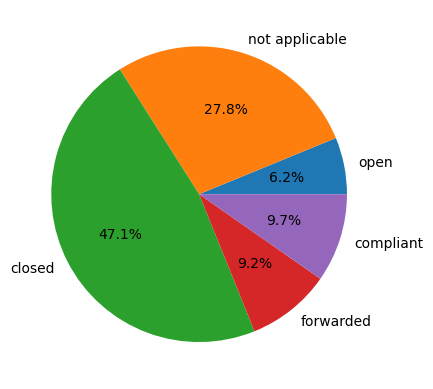
\includegraphics[width = \textwidth/2]{abbildungen/Status.png}
    \caption{Tortendiagramm des Attributs Status}
    \label{fig:StatusPie}
\end{figure}

Als Nächstes werden mithilfe der unique()-Methode alle Ausprägungen der weiteren Attribute überprüft. Beim Quellcode \ref*{lst:ProductUnique} fallen zwei Ausprägungen
auf, diese wurden zur Verdeutlichung in der Ausgabe rot markiert. Die Produktbezeichnung ist bei manchen Fällen \glqq nan\grqq{} oder \glqq /\grqq{} und stellen somit
keine wirklichen Produkte dar. Um die Ursache dafür herauszufinden, ist es sinnvoll, sich die Zeilen anzusehen, in der diese Probleme auftreten. Dafür wird die
loc()-Methode aus der Pandas-Bibliothek genutzt. Diese Methode wird genutzt, um gezielt Datenbereiche eines Dataframes auszuwählen. Zudem können mithilfe dieser Methode
Datenoperationen auf den ausgewählten Daten ausgeführt werden. In Zeile zwei des Quellcodes \ref*{lst:ProductUnique} werden alle Zeilen ausgewählt, die als Produkt
den Wert \glqq nan\grqq{} besitzen. Dabei werden nur die Spalten \glqq Product\grqq{}, \glqq Version\grqq{} und \glqq Path\grqq ausgewählt und zum Schluss
wird die head()-Methode genutzt, um nur die ersten 5 Zeilen zurückzugeben. Die Ausgabe dieser Zeile kann der unteren Tabelle entnommen werden.
In dieser Tabelle wird deutlich, dass die Produktbezeichnung in der Version enthalten ist. 

\begin{lstlisting}[language = python, caption={Ausprägungen des Attributs Product},captionpos=b, label = lst:ProductUnique, floatplacement=H, escapechar={|}]
    print(df['Product'].unique())
    df.loc[df['Product'].isna(), ['Product', 'Version', 'Path']].head()
    ---------------------------------------
    Output:
    ['DCM' 'ACM300' 'Trainguard 200 RBC' 'SICAS ECC' 'SIMIS IS'
    'ETCS Engineering Process' 'CG ETCS Workstation' 'AzS350U' 'TGMT'
    'ACM200' 'Clearguard TCM 100' 'VICOS OC111' 'LED_70_at_Som6'
    'LED_Anzeigemodul' 'LEU S21 MS MC MT 208-233_-433_-533'
    'Eurobalise S21 und S22' 'SIMIS W' 'VICOS NCU' 'LED_70' 'LED_136'
    'POM4 S700K BSG9' 'Key Switch' 'VICOS OC501' 'LZB700M' |\color{red}nan|
    'LEU S21 MS MC MT 208-203_-403_-503' 'Eurobalise S21' |\color{red}'/'| 'DTS'
    'SIMIS LC' 'AC100' 'LEU S21 M ME 208-201_-401']

    Product          Version                                  Path
        NaN  VICOS_S_D_02.14  /23147 ML_KSA_SRO_Line1_Enhancements
        NaN  VICOS_S_D_02.14  /23147 ML_KSA_SRO_Line1_Enhancements
        NaN  VICOS_S_D_02.14  /23147 ML_KSA_SRO_Line1_Enhancements
        NaN  VICOS_S_D_03.00                     /55525_ML_HU_KLBA
        NaN  VICOS_S_D_03.00                     /55525_ML_HU_KLBA
\end{lstlisting}

Die Anwendungsregeln zum Produkt \glqq VICOS\_S\_D\grqq{} liegen in der \ac{DOORS}-Datenbank in Modulen unter dem Pfad: /RA Application Conditions/03\_PG\_OCS/Service and diagnostic systems.
Dieser Pfad weicht von der Ordnerstruktur, die in Kapitel \ref*{chap:DataPraxisprojekt} beschrieben wurde, ab. Es fehlt hier der Ordner mit dem Namen des Produkts.
Stattdessen enthält hier das Modul sowohl den Namen des Produkts als auch seine Version. Deshalb müssen die Einträge, die als Produkt den Wert \glqq nan\grqq{} besitzen,
überarbeitet werden. 

\begin{lstlisting}[language = python, caption={Eintragen der korrekten Produkt- und Versionsbezeichnung},captionpos=b, label = lst:UpdateProduct, floatplacement=H]
    df.loc[df['Version'].str.contains('VICOS_S_D'), 'Product'] = 'VICOS_S_D'
    df.loc[df['Version'].str.contains('VICOS_S_D'), 'Version'] = df['Version'].str[-5:]  
\end{lstlisting}

In den beiden Zeilen im Quellcode \ref*{lst:UpdateProduct} werden alle Zeilen überarbeitet, deren Versionsbezeichnung \glqq VICOS\_S\_D\grqq{} enthält.
Alle gefundenen Zeilen bekommen als Produkt den korrekten Wert \glqq VICOS\_S\_D\grqq{} zugeordnet. Die Versionsbezeichnung besteht aus den letzten 5 Zeichen
der Spalte \glqq Version\grqq{} aus der Tabelle im Quellcode \ref*{lst:ProductUnique}. Deshalb wird nur ein Teil der ursprünglichen Versionsbezeichnung
beibehalten. str[-5:] sorgt nämlich dafür, dass nur die letzten 5 Zeichen der Zeichenkette genutzt werden.

Dasselbe Verfahren wird auch für die Fälle durchgeführt, die als Produkt den Wert \glqq /\grqq{} besitzen. Dieser Sonderfall tritt bei 147 bewerteten Anwendungsregeln
aus zwei ungarischen Projekten auf.
Einige Anwendungsregeln stammen nicht aus dem Projekt RA Application Conditions, sondern vermutlich aus einem anderen Projekt oder sie sind speziell 
für diese beiden Projekte. Die ausgehenden Links der Objekte können über die grafische Oberfläche von \ac{DOORS} verfolgt werden, bei diesen beiden Projekten
wird das Zielobjekt aber aufgrund mangelnder Rechte nicht angezeigt, wie in Abbildung \ref{fig:LockedData} gesehen werden kann. 

\begin{figure}[H]
    \centering
    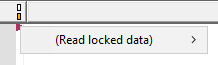
\includegraphics[width = \textwidth/2]{abbildungen/LockedData.PNG}
    \caption{Link auf gesperrte Daten}
    \label{fig:LockedData}
\end{figure}


\section{Sammeln zusätzlicher Daten}
\label{chap:DatenSammeln}
Wie in Kapitel \ref*{chap:DataPraxisprojekt} bereits erwähnt, besteht die Möglichkeit über eine Access-Datenbank noch weitere Daten über die Projekte zu sammeln.
Aus den Inhalten dieser Access-Datenbank wird jeden Tag eine XML-Datei erstellt, welche ebenfalls in das Python-Skript mit der Pandas-Bibliothek importiert werden kann.
In dieser XML-Datei kann dann nach den Projekten aus dem Datensatz gesucht werden und der Datensatz kann dann mit den Daten aus der XML-Datei erweitert werden.
Zunächst wird eine Liste erstellt, die alle eindeutigen Projekte aus dem Datensatz enthält. Diese Liste wird dann verwendet, um eine Schleife durchzuführen, 
in der jeder Projektname nacheinander durchlaufen wird. In der Schleife wird für jedes Projekt der Eintrag aus der Access-Datenbank gesucht.
Dabei muss der Eintrag drei Bedingungen erfüllen:
\begin{enumerate}[topsep=0pt,itemsep=-1ex,partopsep=1ex,parsep=1ex]
    \item \glqq Type\grqq{} muss den Wert \glqq Real\grqq{} besitzen
        \begin{itemize}[itemindent=0cm]
            \item Projekte mit dem \glqq Type\grqq{} \glqq Real\grqq{} befinden sich in der Projektabwicklungsphase
        \end{itemize}
    \item \glqq Location\grqq{} muss den Wert \glqq BWG\grqq{} besitzen
        \begin{itemize}[itemindent=0cm]
            \item \glqq BWG\grqq{} steht hierbei für die \ac{RM} Datenbank Braunschweig
        \end{itemize}
    \item \glqq Offset\grqq{} muss den Wert \glqq path\grqq{} besitzen
        \begin{itemize}[itemindent=0cm]
            \item stellt sicher, dass der Eintrag zum richtigen Projekt gehört
            \item In einem Land existieren mehrere Projekte mit demselben Namen, im Datensatz ist damit jedoch ein bestimmtes Projekt gemeint, die Namen mussten hier anonymisiert werden
        \end{itemize}
\end{enumerate}
Das Prüfen dieser Bedingungen ist eingebettet in einen try-except-Block. Der try-except-Block sorgt dafür, dass eine Fehlermeldung auftritt, falls in der Access-Datenbank ein Eintrag nicht gefunden wird.
Wenn hingegen ein Eintrag gefunden wird, dann wird die erste gefundene Zeile in einer Variable \glqq result\grqq{} gespeichert. Quellcode \ref*{lst:ImportAccess} zeigt den Code, um diese Schritte durchzuführen.
\begin{lstlisting}[language = python, caption={Importieren der Access-Datenbank},captionpos=b, label = lst:ImportAccess, floatplacement=H]
    paths = df['Path'].unique()
    accessDB = pd.read_xml(".../Input_BWG_Combined_Access.xml")
    for path in paths:
        try:
            if(path == "..."):
                result = accessDB.loc[(accessDB['Type'] == "Real") 
                & (accessDB['Location'] == "BWG") 
                & (accessDB['Offset'] == "...")].iloc[0]
            else:
                result = accessDB.loc[(accessDB['Type'] == "Real") 
                & (accessDB['Location'] == "BWG") 
                & ((accessDB['Offset'] == str(path)) | (accessDB['Offset'] == (str(path) + "/")))].iloc[0]           
        except:
            print(str(path) + " has no entry in the AccessDB!")
\end{lstlisting}
\glqq result\grqq{} enthält nun alle Attribute über das Projekt, die in der Access-Datenbank vorhanden sind. Diese relevanten Informationen müssen nun dem ursprünglichen 
Datensatz hinzugefügt werden. Noch in derselben Schleife wie im Quellcode \ref*{lst:ImportAccess}, werden dem Datensatz neue Spalte hinzugefügt und mit den Werten aus der 
Access-Datenbank gefüllt. Quellcode \ref*{lst:addData} zeigt in Zeile drei ein Beispiel dafür. Durch diese Zeile werden alle Zeilen aus dem Datensatz aktualisiert, 
die in der \glqq Path\grqq{}-Spalte den aktuellen \glqq path\grqq{}-Wert haben. Der Wert der neuen Spalte wird dabei aus der entsprechenden Spalte von \glqq result\grqq{} übernommen.
Dieser Schritt wird ebenfalls für die anderen Spalten aus der Access-Datenbank ausgeführt. Zum Schluss wird noch die Versionsbezeichnung angepasst. 
Es kann der Fall auftreten, dass zwei verschiedene Produkte dieselbe Versionsbezeichnung besitzen, zum Beispiel \glqq 2\grqq{} oder \glqq 01.5\grqq{}. Um das zu verhindern,
wird vor die Versionsbezeichnung noch der Name des Produkts gestellt, damit sich Versionsbezeichnungen von verschiedenen Produkten nicht mehr gleichen können.
\begin{lstlisting}[language = python, caption={Erweiterung des Datensatzes},captionpos=b, label = lst:addData, floatplacement=H]
    for path in paths:
        #...
        df.loc[df['Path'] == str(path), 'Project_category']
        = result['Project_category']
        #...
        df['ProductVersion'] 
        = df["Product"].str.cat(df["Version"], sep = "-")
\end{lstlisting}
Das Ergebnis dieser Schritte ist ein Datensatz in Form eines Dataframes mit 14.572 Zeilen und 11 verschiedenen Spalten. Diese zusätzlichen Daten wurden gesammelt, um Ähnlichkeiten von Projekten 
nutzen zu können. Je stärker sich Projekte ähneln, desto eher werden die Anwendungsregeln der Projekte ähnlich bewertet. Die Spalten dieses Dataframes sind die folgenden und dienen, bis auf die 
Spalte \glqq Text\grqq{}, als Datensatz für das Anlernen des \ac{KI}-Modells:
\begin{description}[style=multiline,leftmargin=4cm,font=\bfseries, nolistsep]
    \item[Text] Text der Anwendungsregel
    \item[Product] Name des Produkts
    \item[ProductVersion] Version des Produkts
    \item[Project\_name] Name des Projekts, das die Anwendungsregel bearbeiten musste
    \item[section] Sektion, die das Projekt durchführt, zum Beispiel ML für MainLine oder MT für MassTransit
    \item[Project\_category] Kategorie des Projekts, gibt Aufschluss über die Größe eines Projekts
    \item[BS] Business Segment, in dem das Projekt angesiedelt ist
    \item[RU] Region, in der das Projekt durchgeführt wird
    \item[ProjectYear] Jahr, in dem das Projekt gestartet wurde
    \item[Status] Status der Anwendungsregel
    \item[Statement] Begründung zum Status
\end{description} 

Eine weitere Möglichkeit zur Erzeugung weiterer Daten aus dem bestehenden Datensatz wäre die Data Augmentation. Bei diesem Verfahren werden die bestehenden Daten 
leicht abgeändert, damit weitere Daten synthetisch erstellt werden können, was zu einem größeren Datensatz führt. Diese Praxis wird häufig im Bereich der Computer Vision,
also dem \glqq maschinellen Sehen\grqq{}, genutzt. Computer Vision beschäftigt sich mit der Verarbeitung von Bildern und Videos, weshalb dabei die Datensätze 
aus Bildern und Videos bestehen. Auf den Daten können dann verschiedene Transformationen ausgeführt werden, zum Beispiel kann ein Bild gespiegelt oder gedreht werden, um aus 
einem Bild mehrere zu erzeugen \cite[vgl. S.184f.]{DL_PY}. In dem in dieser Arbeit beschriebenem Anwendungsfall bietet sich Data Augmentation jedoch nicht an. Da der Datensatz überwiegend
aus kategorischen Attributen besteht, müssten einige Kategorien andere Werte bekommen, um aus den vorhandenen Daten weitere zu erzeugen. Dies könnte zum Beispiel dazu führen,
dass eine Zeile im Datensatz, die beispielsweise zu einem Projekt, das eigentlich der Kategorie \glqq A\grqq{} zugehört, unterschiedlichen Kategorien zugeordnet wird, 
was dann aber zu einem Widerspruch im Datensatz führen könnte. Zudem könnten durch das Manipulieren des Datensatzes zufällige Strukturen und Zusammenhänge erzeugt werden,
die in der Realität nicht existieren. Da der Datensatz relativ klein ist, könnte ein \ac{NN} dann diese falschen Strukturen erkennen und diese lernen. Dies wäre kritisch zu betrachten,
da Anwendungsregeln sicherheitsrelevant sein können. Deshalb wurde in dieser Arbeit davon abgesehen, dieses Verfahren zu verwenden.

\section{Codierung der Attribute}
Im nächsten Schritt muss der Datensatz in eine Form gebracht werden, die für das Anlernen eines \ac{KI}-Modells geeignet ist. Die ausgewählten Attribute stellen alle Kategorien in 
Textform oder als Jahreszahl dar. Beide Darstellungsformen sind ungeeignet, um als Trainingsdatensatz zu dienen, da ein \ac{NN} mit numerischen Werten arbeitet. 
Eine Möglichkeit zur Codierung von kategoriellen Attributen ist die One-Hot-Codierung. Dabei wird jeder Ausprägung eines Attributs eine eigene neue Spalte zugeordnet 
und für jede Zeile hat nur eine Spalte den Wert 1, alle anderen Spalten nehmen den Wert 0 an. Die beiden nachfolgenden Tabellen zeigen anhand eines Beispiels die 
One-Hot-Codierung des Attributs \glqq ProjectYear\grqq{}.
\\  
\\
\begin{minipage}[c]{0.5\textwidth}
    \centering
    \begin{tabular}{|c|c|}
        \hline
        \textbf{Text} & \textbf{ProjectYear}\\ \hline
        Text1&2019\\
        Text2&2021\\
        Text3&2022\\
        \hline
    \end{tabular}
    \captionof{table}{Ursprügliche Tabelle}
\end{minipage}
\begin{minipage}[c]{0.5\textwidth}
    \centering
    \begin{tabular}{|c|c|c|c|}
        \hline
        \textbf{Text} & \textbf{2019} & \textbf{2021} & \textbf{2022}\\ \hline
        Text1 & 1 & 0 & 0\\
        Text2 & 0 & 1 & 0\\
        Text3 & 0 & 0 & 1\\
        \hline
    \end{tabular}
    \captionof{table}{Nach One-Hot-Codierung}
\end{minipage}
\\
\\
Um auf den Spalten des Dataframes in Python die One-Hot-Codierung auszuführen, wurde eine neue Funktion geschrieben, die dem Quellcode \ref{lst:OneHot} entnommen werden kann.
Diese Funktion erhält als Parameter einen Dataframe sowie eine Liste an Spalten, auf denen die One-Hot-Codierung durchgeführt werden soll. In einer Schleife iteriert die Funktion 
über jede Spalte, die in der Liste übergeben wurde und prüft anschließend, ob diese Spalte im Dataframe vorhanden ist. Wenn dies der Fall ist, dann wird mithilfe der 
get\_dummies()-Methode aus der Pandas-Bibliothek die One-Hot-Codierung durchgeführt. Anschließend wird die ursprüngliche Spalte aus dem Dataframe entfernt und dafür werden
die neuen codierten Spalten dem Dataframe hinzugefügt. Dafür werden die drop()- und concat()-Methode der Pandas-Bibliothek genutzt, die es ermöglichen Spalten und Zeilen
hinzuzufügen oder zu entfernen \cite{PandasDoc}.

\begin{lstlisting}[language = python, caption={Funktion zur One-Hot-Codierung},captionpos=b, label = lst:OneHot, floatplacement=H]
    def column_one_hot (dataframe, columns): 
        for column in columns:
            if column in dataframe:
                one_hot = pd.get_dummies(dataframe[column])
                dataframe = dataframe.drop(column,axis = 1)
                dataframe = pd.concat([dataframe, one_hot], axis=1)
        return dataframe
\end{lstlisting}

Die Attribute \glqq Product\grqq{} und \glqq ProductVersion\grqq{} stellen hier jedoch einen Sonderfall dar. Aufgrund der One-Hot-Codierung kann in jeder Zeile nur eine Ausprägung
eines Attributs den Wert 1 annehmen, jedoch benutzen Projekte mehrere Produkte und verschiedene Produktversionen. Deshalb muss der Datensatz für diese beiden Attribute nochmal 
überarbeitet werden. Zunächst wird über alle Projekte und Produkte iteriert. Für jedes Produkt wird nun geprüft, ob es in einem Projekt vorhanden ist. Wenn dies der Fall ist,
dann wird der Wert für dieses Produkt in jeder Zeile des Projekts auf eins gesetzt. Äquivalent wird mit dem Attribut \glqq ProductVersion\grqq{} verfahren. 

\begin{lstlisting}[language = python, caption={Anpassung der Spalte \glqq Product\grqq},captionpos=b, label = lst:ProductOneHot, floatplacement=H]
    df = column_one_hot(df, ['Product'])
    for project in projects:
        for product in products:
            df.loc[df['Project_name'] == project, product] = 1 if 
            (df.loc[df['Project_name'] == project][product].sum()) >= 1 else 0
    df = column_one_hot(df, ['ProductVersion', 'Project_name', 'section',
    'Project_category', 'BS', 'RU', 'ProjectYear'])
    ---------------------------------------
    Output:
    (14572, 180)
\end{lstlisting}

Nachdem die beiden Attribute korrekt codiert wurden, können die restlichen Attribute ebenfalls codiert werden, wie im Quellcode \ref*{lst:ProductOneHot} gezeigt wird.
Aus den ursprünglichen 11 Spalten wurden nach der Codierung der Attribute 180 verschiedene Spalten.

Eine Variante der One-Hot-Codierung ist der One-Hot-Hashing-Trick, der sich anbietet, wenn die Anzahl an Attributen in einem Datensatz zu hoch ist. Anstatt jede Ausprägung
eines Attributs als neue Spalte zu definieren, kann auch eine Hashfunktion genutzt werden, um die Ausprägungen abzubilden. François Chollet nutzt diese Variante
der One-Hot-Codierung bei der Codierung von Wörtern und Zeichen. In seinem Beispiel codiert er die 1000 am häufigsten vorkommenden Wörter \cite[vgl. S.236]{DL_PY}. Da der Datensatz in dieser Arbeit aber 
nicht über so viele verschiedene Spalten verfügt, wurde diese Variante der One-Hot-Codierung hier nicht genutzt.

Neben den beiden Varianten existieren noch weitere Möglichkeiten zur Codierung von kategorischen Attributen. Ein weiteres Beispiel wäre das Label-Encoding. Dabei wird jeder Ausprägung eines Attributs
ein eindeutiger Integer-Wert zugeordnet. Die nachfolgenden Tabellen zeigen ein Beispiel für das Label-Encoding eines Attributs. Dem Produkt \glqq SICAS ECC\grqq{} wird dabei der Wert 0 zugeordnet,
dem Produkt \glqq LZB700m\grqq{} 1 und so weiter. 
\\
\\
\begin{minipage}[c]{0.5\textwidth}
    \centering
    \begin{tabular}{|c|c|}
        \hline
        \textbf{Text} & \textbf{Product}\\ \hline
        Text1 & SICAS ECC\\
        Text2 & LZB700M\\
        Text3 & SIMIS IS\\
        \hline
    \end{tabular}
    \captionof{table}{Ursprügliche Tabelle}
\end{minipage}
\begin{minipage}[c]{0.5\textwidth}
    \centering
    \begin{tabular}{|c|c|c|c|}
        \hline
        \textbf{Text} & \textbf{Product} \\ \hline
        Text1 & 0\\
        Text2 & 1\\
        Text3 & 2\\
        \hline
    \end{tabular}
    \captionof{table}{Nach Label-Encoding}
\end{minipage}
\\
\\
Im Vergleich zur One-Hot-Codierung besteht hier der Vorteil, dass nicht für jede Ausprägung eine neue Spalte hinzugefügt wird und 
die Dimension des Datensatzes somit nicht größer wird. Der entscheidende Nachteil des Label-Encodings tritt jedoch auf, wenn die Ausprägungen nicht in einer Beziehung zueinander stehen.
Durch das Zuweisen von aufsteigenden Integer-Werten erweckt diese Art der Codierung den Eindruck, dass die Beziehung \glqq SICAS ECC\grqq{} < \glqq LZB700m\grqq{} < \glqq SIMIS IS\grqq{} besteht,
obwohl das gar nicht der Fall ist. Deshalb wurde in dieser Arbeit das Label-Encoding verworfen und stattdessen die One-Hot-Codierung genutzt.


\section{Aufteilung des Trainingsdatensatzes}
\label{chap:Trainingssplit}
Nachdem die Attribute codiert wurden und der Datensatz somit in eine Form gebracht wurde, die zum Anlernen eines \ac{KI}-Modells geeignet ist, 
muss nun als Nächstes eine Aufteilung in Trainings- und Testdaten sowie in Eingabe- und Ausgabewerte erfolgen. Da die Bewertung einer Anwendungsregel
unabhängig von der Bewertung anderer Anwendungsregeln ist, darf das \ac{KI}-Modell nur mit den Bewertungen zu der spezifischen Anwendungsregel angelernt werden.
Wie Abbildung \ref*{fig:ARMenge} jedoch zeigt, wurden nur 38 Anwendungsregeln mehr als zehnmal bewertet, die allermeisten Anwendungsregeln wurden nur weniger als 
fünfmal bewertet. Das sorgt dafür, dass beim \ac{KI}-Modell mit Überanpassung gerechnet werden muss, da der Datensatz zu klein ist.
\begin{figure}[H]
    \centering
    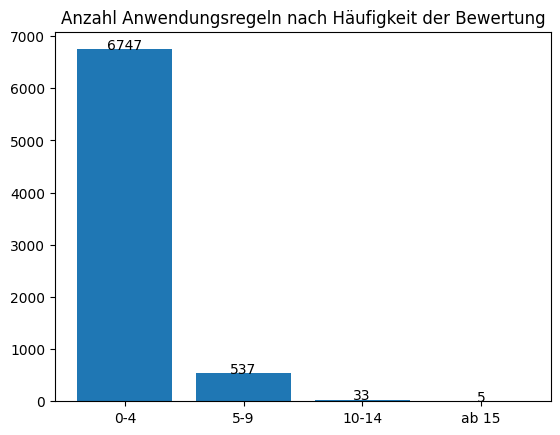
\includegraphics[width = \textwidth]{abbildungen/BalkenAR.png}
    \caption{Säulendiagramm zur Häufigkeit der Bewertung von Anwendungsregeln}
    \label{fig:ARMenge}
\end{figure}

Um den Datensatz auf die Bewertungen von Anwendungsregeln zu beschränken, welche gerade bewertet werden soll, wurde zur Demonstration dieses Schritts 
beispielhaft die Anwendungsregel ausgewählt, welche am häufigsten im Datensatz vorhanden war. Der Quellcode \ref*{lst:defTraining} zeigt den benötigten Code-Ausschnitt,
um diese Schritte durchzuführen.

\begin{lstlisting}[language = python, caption={Definieren des Trainingsdatensatzes},captionpos=b, label = lst:defTraining, floatplacement=H]
df_training = df
text = "Zur Anschaltung des Antriebes in der Außenanlage muessen Signalkabel nach VDE 0816/2 oder Kabel mit vergleichbaren Eigenschaften verwendet werden. Die Verlegevorschriften des Kabels sind einzuhalten."
df_training = df_training.loc[df_training['Text'] == text]

trainX = drop_columns(df_training, ['Status', 'Text', 'Statement'])
trainYStatus = drop_column(column_one_hot(df_training[['Text', 'Status']], ['Status']), "Text")
trainYStatement = drop_column(column_one_hot(df_training[['Text', 'Statement']], ['Statement']), "Text")
\end{lstlisting}

Zeile 2 des Quellcodes \ref*{lst:defTraining} speichert den beispielhaft ausgewählten Text einer Anwendungsregel in eine Variable. Bei der späteren Anwendung würde dieser Text
aus dem Modul in \ac{DOORS} extrahiert werden. In der nächsten Zeile wird der Datensatz auf die Zeilen beschränkt, die als Text den ausgewählten Text besitzen.
Die letzten drei Zeilen werden für die Aufteilung in Eingabe- und Ausgabewerte benötigt. Alle Spalten, bis auf die beiden Ausgabewerte \glqq Status\grqq{} und 
\glqq Statement\grqq{} sowie der Text der Anwendungsregel, stellen die Eingabewerte dar. Die beiden Ausgabewerte mussten in jeweils eigene Dataframes aufgeteilt werden, 
der Grund dafür wird in Kapitel \ref*{chap:TrainNN} beschrieben.

Nun sind die Daten korrekt codiert und aufgeteilt in einen Trainingsdatensatz mit getrennten Ein- und Ausgabewerten. Der Testsplit wird beim Anlernen definiert, näheres dazu ebenfalls in 
Kapitel \ref*{chap:TrainNN}.
